\section{Funções}
\label{sec:functions}

Quando você se vê fazendo a mesma tarefa diversas vezes, talvez seja um bom momento para criar uma função reutilizável. Uma função, como você aprendeu na seção de Fechamentos, é algo escrito entre chaves. David Touretzky introduz a ideia de função da seguinte forma: “pense na função como uma caixa através da qual os dados passam. Essa função opera sobre os dados de alguma forma e o resultado é o que passa para fora.” \footnote{Touretzky, David. COMMON LISP: A Gentle Introduction to Symbolic Computation. The Benjamin/Cummings Publishing Company, Inc, 1990, p. 1. Este é o livro que inspirou o título original em inglês deste tutorial.}

\begin{figure}[h]
\centerline{\framebox{
	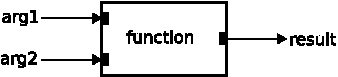
\includegraphics[scale=0.9]{fig-function-box.pdf}}}
\caption{Ideia geral de uma função.}
\label{fig:function-box}
\end{figure}

A primeira linha no exemplo abaixo define a função, atribuindo-a à variável \texttt{f}. A segunda linha coloca a função para trabalhar.

 
\begin{lstlisting}[style=SuperCollider-IDE, basicstyle=\scttfamily\footnotesize]
f = { 2 + 2 }; // define a função
f.value; // colocar a função para trabalhar
\end{lstlisting}
 
A função acima não é terrivelmente útil, pois apenas sabe fazer uma única coisa (somar 2 e 2). Normalmente você vai querer definir funções que podem dar diferentes resultados dependendo dos argumentos de entrada que você forneça. Nós usamos a palavra-chave \texttt{arg} para especificar as entradas que uma função pode aceitar. O exemplo abaixo é mais parecido com o desenho da figura \ref{fig:function-box}.
 
\begin{lstlisting}[style=SuperCollider-IDE, basicstyle=\scttfamily\footnotesize]
f = {arg a, b; ["a mais b", a+b, "a vezes b", a*b].postln}; // define função
f.value(3, 7); // agora você pode dois números quaisquer como argumentos para a função
f.value(10, 14);

// Compare:
~sillyRand = rrand(0, 10); // não é uma função
~sillyRand.value; // execute diversas vezes
~sillyRand2 = {rrand(0, 10)}; // é uma função
~sillyRand2.value; // execute diversas vezes
\end{lstlisting}
 
Como um último exemplo, aqui está uma função muito útil.
 
\begin{lstlisting}[style=SuperCollider-IDE, basicstyle=\scttfamily\footnotesize]
// Use esta função para decidir como passar seus dias de verão

(
~oQueFazer = { 
var hoje, nomeDoDia, acoes;
	hoje = Date.getDate.dayOfWeek;
	nomeDoDia = 
	case
	{hoje==0} {“Domingo”}
	{hoje==1} {“Segunda”}
	{hoje==2} {"Terça”}
	{hoje==3} {“Quarta”}
	{hoje==4} {“Quinta”}
	{hoje==5} {“Sexta”}
	{hoje==6} {"Sábado”};
	acoes = [“jogar bumerangue”, “queda de braço“, “subir escadas”, “jogar xadrez“, “hóquei subaquático“, “atirar ervilhas“, “longa soneca"];
	"Ah, " ++ nomeDoDia ++ "...! " ++ “Que ótimo dia para " ++ acoes.choose;
};
)

// Execute pela manhã
~oQueFazer.value;
\end{lstlisting}

\bigskip
\todo[inline, color=green!40]{ DICA: Outra notação comum para declarar argumentos no início de uma Função é: \texttt{f = \{|a, b| a + b\}}. Isso é equivalente a \texttt{f = \{arg a, b; a + b\}}} 

